\documentclass[11pt]{beamer}  %% versione proiettore
%%\documentclass[11pt,handout]{beamer} %% versione stampa
\usepackage{lucidiJb-2ed}

\usepackage{relsize}

\mode<article>
{
  \usepackage{fullpage}
  \usepackage{hyperref}
}

\mode<presentation>
{
  \setbeamertemplate{background canvas}[vertical shading][bottom=red!10,top=blue!10]
  \usetheme{Ethereum}
  \usefonttheme[onlysmall]{structurebold}
}

\subtitle{Learning Ethereum}
\title{Smart Contracts}
\institute{Universit\`a di Verona, Italy}
\date{January 2020}

\setbeamercovered{invisible}

\def\codesize{\smaller}
\def\<#1>{\codeid{#1}}
\newcommand{\codeid}[1]{\ifmmode{\mbox{\codesize\ttfamily{#1}}}\else{\codesize\ttfamily #1}\fi}

\begin{document}

\begin{frame}
  \titlepage
\end{frame}

\begin{frame}\frametitle{A smart contract is\ldots}

  \begin{itemize}
  \item a computer program (not \emph{smart} nor \emph{a contract})
  \item immutable
  \item deterministic
  \item operating on restricted data
  \item running on a decentralized world computer
  \end{itemize}

  In Ethereum:
  \begin{itemize}
  \item compiled into EVM bytecode
  \item installed by sending a special transaction to address \<0x0>
  \item its code can be deleted if it contains a \<SELFDESTRUCT> bytecode
  \item has no keys
  \item who installs it gets no automatic privileges
  \item runs after a transaction initiated by an EOA
    \begin{itemize}
    \item or a chain of transactions initiated by an EOA
    \item no parallelism, no background processing
    \end{itemize}
  \item transactions are atomic
  \end{itemize}
  
\end{frame}

\begin{frame}\frametitle{Back to our first Solidity example}
  \begin{center}
    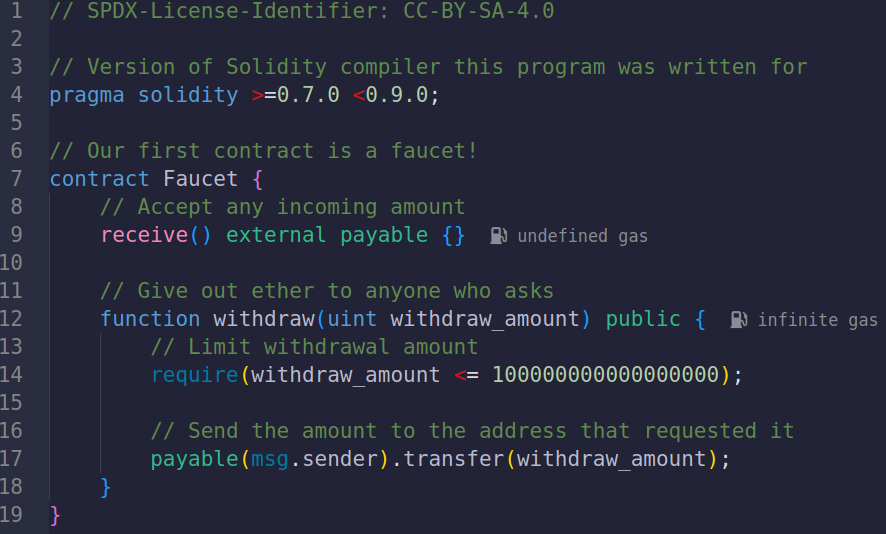
\includegraphics[width=\textwidth,clip=false]{pictures/faucet_sol.png}
  \end{center}
\end{frame}

\begin{frame}[fragile]\frametitle{ABI -- from Remix or from \<solc>}

{\scriptsize\begin{verbatim}
[
  {
    "payable": true,
    "stateMutability": "payable",
    "type": "fallback"
  },
  {
    "constant": false,
    "inputs": [
      {
        "internalType": "uint256",
        "name": "withdraw_amount",
        "type": "uint256"
      }
    ],
    "name": "withdraw",
    "outputs": [],
    "payable": false,
    "stateMutability": "nonpayable",
    "type": "function"
  }
]
\end{verbatim}}
\end{frame}

\begin{frame}[fragile]\frametitle{Select a compiler version}

  \begin{greenbox}{Add a pragma directive}
    \verb!pragma solidity ^0.4.19! requires to compile with a compiler for version $0.4.x$ with $x\ge 19$.
  \end{greenbox}

\end{frame}

\begin{frame}\frametitle{Basic Solidity types}
  \begin{greenbox}{\<bool>}
    with constants \<true> and \<false> and usual operators
  \end{greenbox}
  \bigskip
  \begin{greenbox}{\<int>, \<unint>}
    signed or unsigned, witgh usual operators, in increments of 8 bit size:
    \<uint8>, \<uint16>, \<int24>\ldots. Without specification, they stand for
    \<int256> and \<unint256>, respectively
  \end{greenbox}
  \bigskip
  \begin{greenbox}{\<fixed>$M\times N$, \<ufixed>$M\times N$}
    fixed point arithmetic, signed or unsigned, $M$ bits, $N$ decimals
    after th epoint
  \end{greenbox}
  \bigskip
  \begin{greenbox}{\<address>}
    a 20-bytes Ethereum address, with members \<balance> and \<transfer>
  \end{greenbox}

\end{frame}

\begin{frame}[fragile]\frametitle{Basic Solidity types}

  \begin{greenbox}{\<bytes>$N$}
    fixed-size array of bytes, of length $N$
  \end{greenbox}

  \bigskip

  \begin{greenbox}{\<bytes> or \<string>}
    variable-sized arrays of bytes
  \end{greenbox}

  \bigskip

  \begin{greenbox}{Arrays}
    \<uint32[][5]> is a fixed size array of five dynamic
    arrays of $32$ bits unsigned integers
  \end{greenbox}

  \bigskip

  \begin{greenbox}{Enum's}
\begin{verbatim}
enum NAME { A, B, ... }
\end{verbatim}
  \end{greenbox}

\end{frame}

\begin{frame}[fragile]\frametitle{Basic Solidity types}

  \begin{greenbox}{Struct's}
\begin{verbatim}
struct pair {
  int16 x;
  unint8 y;
}
\end{verbatim}
  \end{greenbox}

  \bigskip

  \begin{greenbox}{Mappings}
\begin{verbatim}
mapping(address => unint256) balances;
\end{verbatim}
  \end{greenbox}

\end{frame}

\begin{frame}[fragile]\frametitle{Unit multipliers}

  \begin{greenbox}{Time units: \<seconds>, \<minutes>, \<hours>, \<days>}
\begin{verbatim}
uint delay = 3 hours;
\end{verbatim}
  \end{greenbox}

  \bigskip

  \begin{greenbox}{Ether units: \<wei>, \<finney>, \<szabo>, \<ether>}
\begin{verbatim}
require(withdraw_amount <= 0.1 ether);
\end{verbatim}
  \end{greenbox}

\end{frame}

\begin{frame}\frametitle{Transaction information}

  \begin{greenbox}{Structures \<msg> and \<tx> are computed from the transaction request}
    \begin{description}
    \item[\<msg.sender>] the address that sent the transaction
    \item[\<msg.value>] the ether sent along the transaction
    \item[\<msg.gasleft>] what remains to consume of the gas limit
    \item[\<msg.data>] the data payload of the transaction
    \item[\<msg.sig>] the first four bytes of \<msg.data> (method selector)
    \item[\<tx.gasprice>] the gas price used
    \item[\<tx.origin>] the address of the \alert{originating} EOA
    \end{description}
  \end{greenbox}

\end{frame}

\begin{frame}\frametitle{\<msg.sender> vs \<tx.origin>}

  \begin{center}
    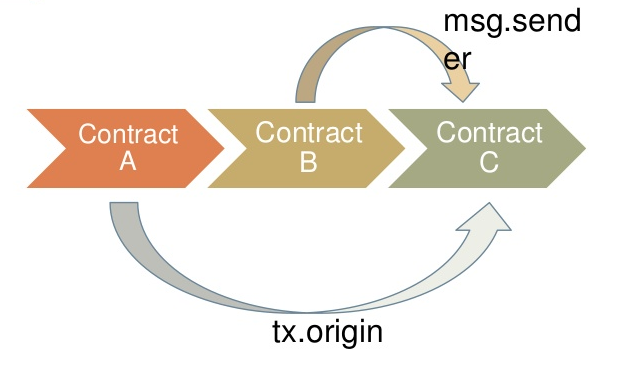
\includegraphics[width=\textwidth,clip=false]{pictures/sender-origin.png}
  \end{center}

\end{frame}

\begin{frame}\frametitle{Block information}

  \begin{greenbox}{The structure \<block> is constructed by the miner}
    \begin{description}
    \item[\<block.coinbase>] the address of the miner
    \item[\<block.difficulty>] the proof of work difficult
    \item[\<block.gaslimit>] the maximum gas spent in the block
    \item[\<block.number>] the current block height
    \item[\<block.timestamp>] the mining time
    \end{description}
  \end{greenbox}

\end{frame}

\begin{frame}\frametitle{Members of an address}

  \begin{greenbox}{}
    \begin{description}
    \item[\<address.balance>] the balance of the address (EOA or contract),
      such as \<address(this).balance>
    \item[\<address.transfer(x)>] sends $x$ wei to the address; throws an exception in case of
      failure
    \item[\<address.send(x)>] as \<transfer>, but returns \<false> in case of failure
    \item[\<address.call(p)>] sends a method transaction to the address, with the given
      payload; returns \<false> in case of failure
    \item[\<address.callcode(p)>] sends a method transaction to the address, with the given
      payload; runs in the scope of the caller; returns \<false> in case of failure
    \item[\<address.delegatecode(p)>] sends a method transaction to the address, with the given
      payload, but keeps \<msg.sender> and \<msg.value> unchanged;
      runs in the scope of the caller; returns \<false> in case of failure
    \end{description}
  \end{greenbox}
  
\end{frame}

\begin{frame}\frametitle{Example of function call}
  \begin{center}
    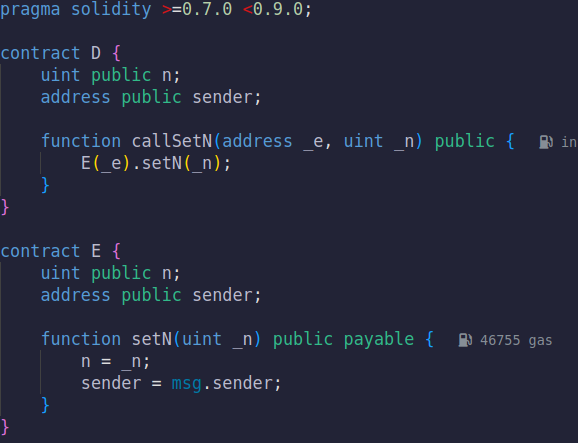
\includegraphics[scale=0.3,clip=false]{pictures/normal-call.png}
  \end{center}

  Calling \<d.callSetN(e, 42)>:
  \begin{itemize}
  \item \<e.n> will become $42$
  \item \<e.sender> will become \<d>
  \item \<d.n> and \<d.sender> are not modified
  \end{itemize}
\end{frame}

\begin{frame}\frametitle{Example of low-level \<call>}

  \begin{center}
    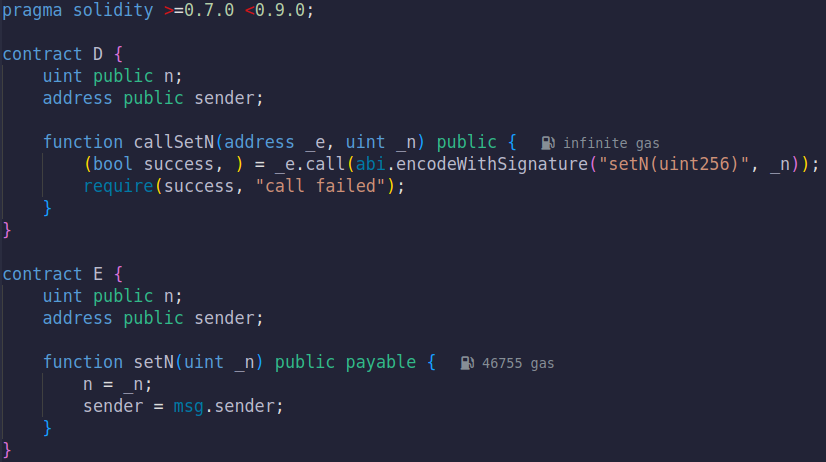
\includegraphics[scale=0.3,clip=false]{pictures/call.png}
  \end{center}

  Calling \<d.callSetN(e, 42)>:
  \begin{itemize}
  \item \<e.n> will become $42$
  \item \<e.sender> will become \<d>
  \item \<d.n> and \<d.sender> are not modified
  \end{itemize}
  
\end{frame}

\begin{frame}\frametitle{Example of a failing low-level \<call>}

  \begin{center}
    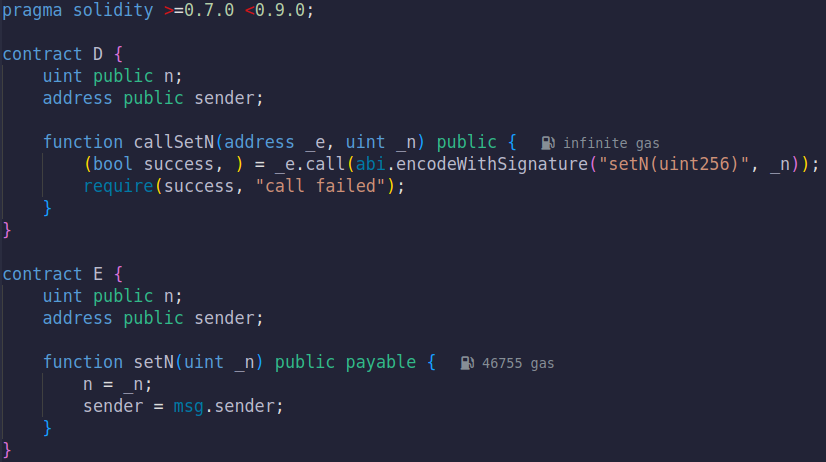
\includegraphics[scale=0.3,clip=false]{pictures/call.png}
  \end{center}

  Calling \<d.callSetN(c, 42)> where \<c> has no \<setN(uint \_n)> function:
  \begin{itemize}
  \item the outer transaction will succeed
  \item the inner \<\_e.call> transaction will fail and be reverted
  \item function \<\_e.call> will return \<false>
  \end{itemize}
  
\end{frame}

\begin{frame}\frametitle{Example of low-level \<callcall>}

  \begin{center}
    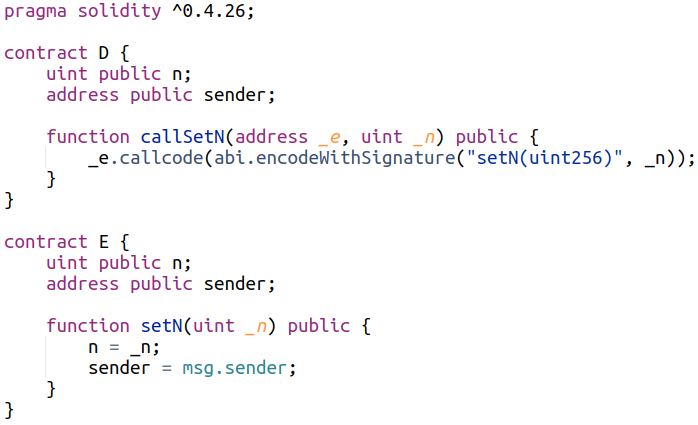
\includegraphics[scale=0.3,clip=false]{pictures/callcode.png}
  \end{center}

  Calling \<d.callSetN(e, 42)>:
  \begin{itemize}
  \item \<d.n> will become $42$
  \item \<d.sender> will become \<d>
  \item \<e.n> and \<e.sender> are not modified
  \end{itemize}
  
\end{frame}

\begin{frame}\frametitle{Example of low-level \<delegatecall>}

  \begin{center}
    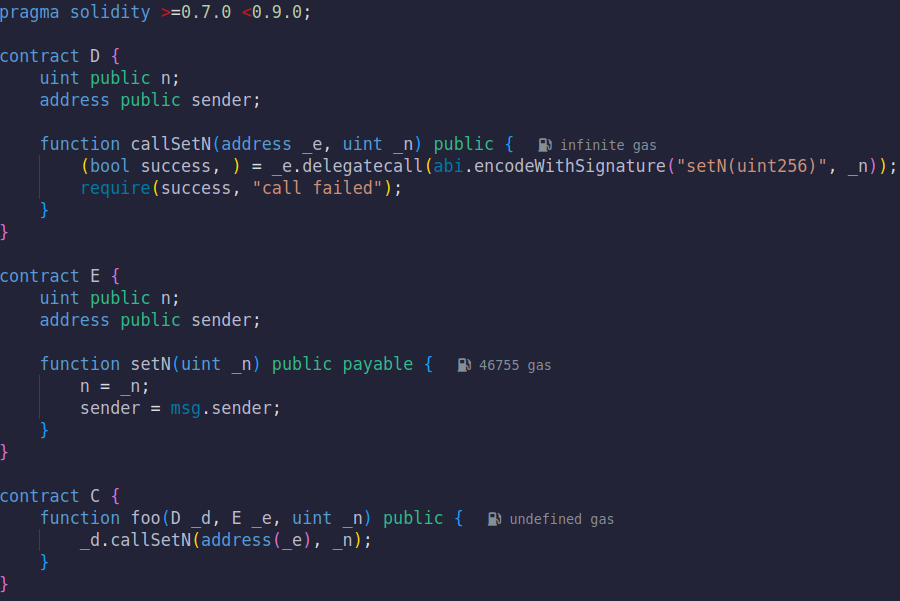
\includegraphics[scale=0.3,clip=false]{pictures/delegatecall.png}
  \end{center}

  Calling \<c.foo(d, e, 42)>:
  \begin{itemize}
  \item \<d.n> will become $42$
  \item \<d.sender> will become \<c>
  \item \<e.n> and \<e.sender> are not modified
  \end{itemize}
  
\end{frame}

\begin{frame}\frametitle{Casts do not fail in Solidity}

  Contract parameter types are just casts:
  \begin{center}
    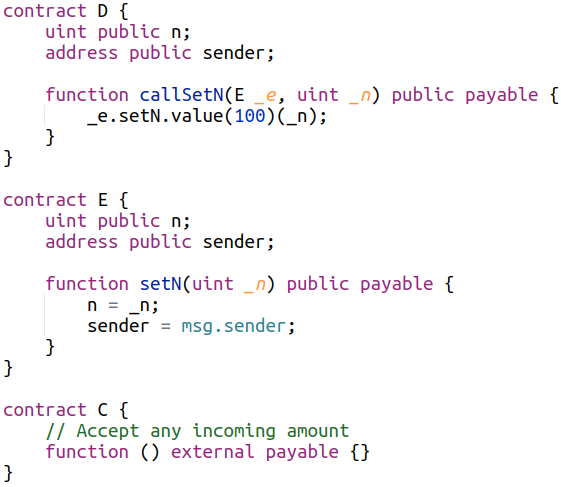
\includegraphics[scale=0.3,clip=false]{pictures/cast-does-not-fail.png}
  \end{center}

  Calling \<d.callSetN(c, 42)>, where \<c> is a \<C>,
  does not fail but calls \<C>'s
  fallback function and transfers all sent value to \<c>!
\end{frame}

\end{document}
